\documentclass[a4paper]{report}
\usepackage[english]{babel}
\usepackage[T1]{fontenc}
\usepackage{comment,fullpage,here,amsfonts,amssymb,amsthm,amsmath,enumerate,array,graphicx} 
\usepackage{lastpage}
\usepackage{fancyhdr,hyperref,bbding}
\usepackage[usenames,dvipsnames]{xcolor}
\usepackage{eso-pic}
\usepackage{biblatex}
\setlength{\parindent}{0cm}
\newcommand{\bu}[1]{\textbf{\underline{#1}}}

\renewcommand{\b}[1]{\textbf{#1}}  % 
\renewcommand{\i}[1]{\textit{#1}}  % Classes and structs
\newcommand{\e}[1]{\emph{#1}}    % File names
\renewcommand{\thesubsection}{(\alph{subsection})}
\renewcommand{\qed}{\hfill \mbox{\raggedright \rule{0.1in}{0.1in}}}
\newcommand{\ooo}{\"{o}}
\newcommand\BackgroundPic{
\put(0,50){\parbox[b][\paperheight]{\paperwidth}{%
\vfill
\centering
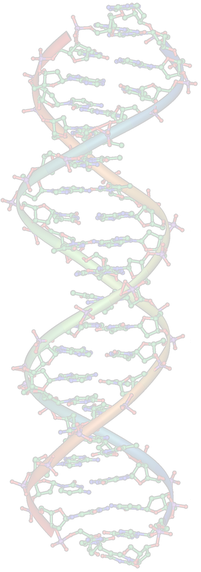
\includegraphics[width=130pt,
keepaspectratio]{img/DNA_Overview2.png}%
\vfill
}}}


\bibliography{refsBFG}
\pagestyle{fancy}
\renewcommand{\headrulewidth}{0.4pt}
\renewcommand{\headheight}{25pt}

\fancypagestyle{plain}{%
    \lhead{BFGraph - Documentation}
    \rhead{Page \thepage\enspace of\enspace  \pageref{LastPage}}
    \renewcommand{\headrulewidth}{0.4pt}
    \renewcommand{\headheight}{25pt}
}


\definecolor{linkcolour}{rgb}{0,0,0.7}
\hypersetup{colorlinks,breaklinks,urlcolor=linkcolour,urlcolor=linkcolour,linkcolor=linkcolour}



\begin{document}
\AddToShipoutPicture*{\BackgroundPic}
\thispagestyle{empty}
\vspace*{110pt}
\begin{center}
\Huge\ \b{Documentation for BFGraph}\\[10pt] \Large A memory efficient De Brujin graph assembler using Bloom Filters
\\[50pt]
\begin{tabular}{c} 
    Pall Melsted\\
    Trausti Saemundsson\\ 
\end{tabular}
\end{center}
\vfill
\large\b{BFGraph Documentation} \hfill \today\\
\normalsize Questions and bug reports: \href{mailto:pmelsted@gmail.com}{pmelsted@gmail.com}
\tableofcontents
\addtocounter{footnote}{-1}
\let\thefootnote\relax\footnotetext{Cover photo is from Wikipedia\cite{wiki:coverphoto}}
\newpage
%\addcontentsline{toc}{chapter}{\protect\numberline{}Introduction}
\chapter{Introduction} 
This is a documentation for the program BFGraph. BFGraph is a De Brujin graph assembler.
Currently it makes the pregraph but does not simplify it like SOAPdenovo\cite{wiki:soap} and Velvet\cite{wiki:velvet}.
It makes the pregraph by using Bloom Filters in contrast to most other assemblers, that use hash tables.
This saves a lot of memory and the result is independent of the false positive rate of the Bloom Filter.\\[2pt]

A Bloom Filter is quite similar to a hash table but. If a Bloom Filter is queried for a specific key,
it answer correctly if the key is not stored but answers incorrectly according to the false positive rate if the key is stored within it.

The first phase of BFGraph makes the pregraph according to a Bloom Filter but then fixes the graph afterwards which makes it
independent of the probabilistic nature of the Bloom Filter. 
The memory usage of BFGraph is a lot lower than that of most other assemblers, and it is compared in the paper about this program.




\chapter{Definitions}
\b{kmer}\cite{wiki:kmer}: string of A,C,G,T which has length $k$ ($k$ is often $31$) \\
\b{twin}: interchange A <-> T and C <-> G in a string and then reverse it \\
\b{contig}: string of A,C,G,T which has length greater or equal to the kmer size\\[8pt]

\chapter{Dependencies}
Inside the program directory are a few programs made by others:

\begin{itemize}
\item \b{sparse\_hash}\cite{sparsehash} is inside the directory google, a memory efficient hash table made by Google
    used in this program for storing common kmers.
\item \b{libdivide}\cite{libdivide} in the file \emph{libdivide.h} is used for fast integer division.
\item \b{kseq}\cite{kseq} in the file \emph{kseq.h} is used for fasta/fastq file reading.
\end{itemize}

\chapter{Usage}
First the program has to be compiled. Run {\verb `make` } to do that.
The directory \e{example} contains two small  read files in fastq format: 
\e{tinyread\_1.fq} and \e{tinyread\_2.fq}.\\[4pt]

Here follows a guide on how to run the program on these two files with one thread and kmer-size 31.
The script \e{example.sh} does the same as described below.

\section{Part I: Filter the reads}
This command filters the reads and saves the result to a new file, \e{example/output/tiny.bf} (it will contain a Bloom Filter).
\begin{verbatim}
$ ./BFGraph filter example/tinyread_*.fq -k 31 -t 1 -o example/output/tiny.bf -n 8000 -N 4000 -v
\end{verbatim}

The parameter \b{-n} is an upper bound of the number of kmers from the read files and the parameter \b{-N} is an upper bound
of the number of \textit{different} kmers from the read files. The parameter \b{-v} is for verbose mode.\\[4pt]

\subsection{Values for -N and -n}  %TODO: Change this part when the estimate program using streaming algorithm has been written
On the TODO list for BFGraph is to write a program to estimate these numbers from the reads. But until it has been written the user has to estimate
them by himself. \\[4pt]

The first number is easy to calculate by hand. The files \e{tinyread\_1.fq} and \e{tinyread\_2.fq} have in total 2000 reads of length $70$.
Since the kmer-size is $31$, we will get $40$ kmers from every read $(70 - 31 + 1=40)$. Thus the number of kmers from the files
is: $40\cdot 2000=8000$. \\[4pt]

\textit{NOTE: These number do not have to be accurate, but the program runs faster if they are close to correct values.} \\[4pt]

We can expect that an average kmer will be seen at least twice so $4000$ is not a bad value for \b{-N}.

\newpage
\section{Part II: Create the contigs}
This phase of the program reads the file \e{example/output/tiny.bf}, which is a Bloom Filter, and creates contigs from the kmers. 
The program must be run with the same kmer-size as the Bloom Filter file was created with, in this case 31.
This command creates the contigs in one thread and saves the results into files with the prefix: \e{example/output/tiny}.
\footnotesize
\begin{verbatim}
$ ./BFGraph contigs example/tinyread_*.fq -k 31 -t 1 -f example/output/tiny.bf -o example/output/tiny -v
\end{verbatim}
\normalsize

\section{Extra: Visualize the De Brujin graph}
For small read files the Python program \e{make\_graph.py} can create a \b{.dot} file with Graphviz\cite{graphviz} 
to visualize the De Brujin graph.

If you ran the commands above you can now run this program with the prefix from Part II above.
\begin{verbatim}
$ ./make_graph.py example/output/tiny
\end{verbatim}

This creates the file \e{example/output/tiny.dot}.\\[4pt]

This file can be read a native \b{.dot} file reader like ZGRViewer\cite{zgr} or converted to \b{.PNG} if Graphviz is installed with the following command:
\begin{verbatim}
$ dot -Tpng example/output/tiny.dot -o example/output/tiny.png
\end{verbatim}







\chapter{Structure of the program}
The file \e{BFGraph.cpp} is compiled into the executable file \e{BFGraph} when `make` is run. 
\e{BFGraph} runs the correct functions based on the input.\\[4pt]
When the command 'filter' is given, the method \i{FilterReads} is called, (implemented in \e{FilterReads.cpp}).\\
When the command 'contigs' is given, the method \i{BuildContigs} is called, (implemented in \e{BuildContigs.cpp}).\\

The program flow is quite similar for those two commands. Parameters are first validated and an appropriate error message is given
on any error. If all the parameters are valid, either \i{FilterReads\_Normal} or \i{BuildContigs\_Normal} is called depending
on the command name. Both those methods go through all the reads (in a while loop) in as many threads as given by the parameter \b{-t}.\\[4pt]

The OpenMP\cite{openmp} library is used for parallel programming in BFGraph.\\[4pt] 





\chapter{Files}

\section{Unused files}
Every file in BFGraph's base directory is used by the program except the following files:

\begin{itemize}
\item \emph{CountBF.hpp}
\item \emph{CountBF.cpp}
\item \emph{DumpBF.hpp}
\item \emph{DumpBF.cpp}
\item \emph{KmerIntPair.hpp}
\item \emph{KmerIntPair.hpp}
\item \emph{bloom\_filter.hpp}
\item \emph{BlockedBloomFilter.hpp}
\end{itemize}

\section{Used files}
The following classes reside in files by a similar name except ContigRef, it is located in \emph{KmerMapper.hpp} and
FastqFile is located in \emph{fastq.hpp}
\subsection{Classes}
\begin{itemize}
\item BloomFilter 
\item CompressedCoverage  
\item CompressedSequence  
\item Contig  
\item ContigRef   
\item FastqFile   
\item Kmer    
\item KmerIterator    
\item KmerMapper  
\end{itemize}

\subsection{Structs}
\begin{itemize}
\item \i{FilterReads\_ProgramOptions} is used as the name indicates to store parameter values from the user 
        for the subcommand \b{filter}, located in \e{FilterReads.cpp}
\item \i{BuildContigs\_ProgramOptions} is used to store parameter values from the user for 
    the subcommand \b{contigs}, located in \e{BuildContigs.cpp}7
\item \i{CheckContig} 
\item \i{FindContig}  
\item \i{MakeContig}
\item \i{NewContig}
\item \i{KmerHash}
\end{itemize}

\chapter{Important methods in the program}


\chapter{Final words}

Thanks.

\vfill

\printbibliography                                                                                                                                   

\end{document}

